\documentclass{beamer}
\usepackage{listings}
\lstset{
%language=C,
frame=single, 
breaklines=true,
columns=fullflexible
}
\usepackage{blkarray}
\usepackage{subcaption}
\usepackage{url}
\usepackage{tikz}
\usepackage{tkz-euclide} % loads  TikZ and tkz-base
%\usetkzobj{all}
\usetikzlibrary{calc,math}
\usepackage{float}
\providecommand{\brak}[1]{\ensuremath{\left(#1\right)}}
\providecommand{\pr}[1]{\ensuremath{\Pr\left(#1\right)}}
\newcommand{\myvec}[1]{\ensuremath{\begin{pmatrix}#1\end{pmatrix}}}
\newcommand\norm[1]{\left\lVert#1\right\rVert}
\renewcommand{\vec}[1]{\mathbf{#1}}
\usepackage[export]{adjustbox}
\usepackage[utf8]{inputenc}
\usepackage{amsmath}
\usepackage{tikz}
\usetikzlibrary{automata, positioning}
\usetheme{Boadilla}

\title{GATE EC 1998 Q1.4}
\author{Nelakuditi Rahul Naga - AI20BTECH11029}
\begin{document}

\begin{frame}
\titlepage
\end{frame}

\begin{frame}
\frametitle{Question}
\begin{block}{GATE EC 1998 Q1.4}
The trigonometric Fourier series of a periodic time function can have only:
\begin{enumerate}
\item cosine terms 
\item sine terms
\item d.c. ,cosine and sine terms
\item d.c. and cosine terms 
\end{enumerate}
\end{block}
\end{frame}

\begin{frame}
\frametitle{Solution}
\begin{block}{Fourier series of a periodic function}
The trigonometric Fourier series of a periodic function $x(t)$ with period $T$ is given by:
\begin{align}
x(t) &= a_{0} + \sum_{k=1}^{\infty}a_{k}\cos{\frac{2\pi kt}{T}} +\sum_{k=1}^{\infty}b_{k}\sin{\frac{2\pi kt}{T}} \\
a_{0} &= \frac{1}{T}{\int_{-\frac{T}{2}}^{\frac{T}{2}}x(t)\, dt} \\
a_{k} &= \frac{2}{T}{\int_{-\frac{T}{2}}^{\frac{T}{2}}x(t)\cos{\frac{2\pi kt}{T}}\, dt} \\
b_{k} &= \frac{2}{T}{\int_{-\frac{T}{2}}^{\frac{T}{2}}x(t)\sin{\frac{2\pi kt}{T}}\, dt} 
\end{align}
\end{block}
The Fourier series of some example functions are demonstrated below.
\end{frame}

\begin{frame}
\frametitle{}
We have a even periodic function having period $2\pi$ defined in $[-\pi,\pi]$ as follows :
\begin{align}
x(t)=  
\begin{cases}
\frac{\pi}{2}+t, & \text{if } -\pi \leq t \leq 0\\
\frac{\pi}{2}-t, & \text{if } 0 < t \leq \pi \nonumber
\end{cases}
\end{align}
The Fourier series of $x(t)$ is determined as follows:
\begin{align}
a_{0} &=\frac{1}{2\pi}\Bigg({\int_{-\pi}^{0}x(t)\, dt}+{\int_{0}^{\pi}x(t)\, dt}\Bigg)=0 \nonumber \\
a_{k} &= \frac{1}{\pi}\Bigg({\int_{-\pi}^{0}x(t)\cos{kt}\, dt}+{\int_{0}^{\pi}x(t)\cos{kt}\, dt}\Bigg) \nonumber = \frac{2(1-(-1)^{k})}{\pi k^{2}}\nonumber \\
b_{k} &= \frac{1}{\pi}{\int_{-\pi}^{\pi}x(t)\sin{kt}\, dt} = 0 \nonumber \\
\implies x(t) &= \frac{4}{\pi}\sum_{k=1}^{\infty}\frac{\cos{(2k-1)t}}{(2k-1)^{2}}
\end{align}
\end{frame}

\begin{frame}
\frametitle{}
\begin{figure}[!ht]
    \centering
    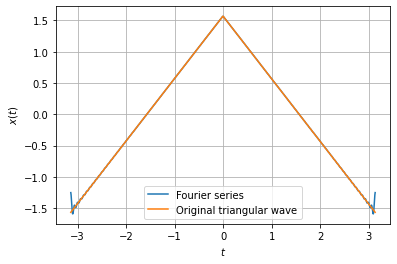
\includegraphics[width=0.8\columnwidth] {Gate_Assignment_4_Fig_1.png}
    \caption{$x(t)$ vs $t$}
    \label{Fourier series of x(t)}
\end{figure}
\end{frame}

\begin{frame}
\frametitle{}
We have a odd periodic function having period $2\pi$ defined in $[0,2\pi]$ as follows :
\begin{align}
x(t)=  
\begin{cases}
1, & \text{if } 0 < t < \pi\\
0, & \text{if } t = 0,\pi,2\pi\\
-1, & \text{if } \pi < t < 2\pi \nonumber
\end{cases}
\end{align}
The Fourier series of $x(t)$ is determined as follows:
\begin{align}
a_{0} &=\frac{1}{2\pi}{\int_{-\pi}^{\pi}x(t)\, dt}=0 \nonumber \\
a_{k} &= \frac{1}{\pi}{\int_{-\pi}^{\pi}x(t)\cos{kt}\, dt} = 0\nonumber \\
b_{k} &= \frac{1}{\pi}\Bigg({\int_{-\pi}^{0}x(t)\sin{kt}\, dt}+{\int_{0}^{\pi}x(t)\sin{kt}\, dt}\Bigg) \nonumber = \frac{2(1-(-1)^{k})}{\pi k}\nonumber \\
\implies x(t) &= \frac{4}{\pi}\sum_{k=1}^{\infty}\frac{\sin{(2k-1)t}}{2k-1}
\end{align}
\end{frame}

\begin{frame}
\frametitle{}
\begin{figure}[!ht]
    \centering
    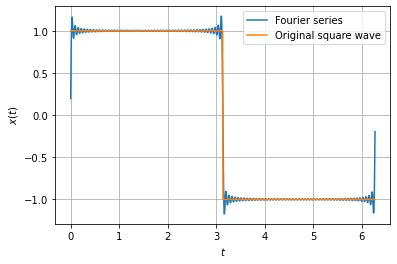
\includegraphics[width=0.8\columnwidth] {Gate_Assignment_4_Fig_2.png}
    \caption{$x(t)$ vs $t$}
    \label{Fourier series of x(t)}
\end{figure}
\end{frame}

\begin{frame}
\frametitle{}
We have a neither even nor odd periodic function having period $2\pi$ defined in $(-\pi,\pi)$ as follows :
\begin{align}
x(t)=  
\begin{cases}
-\pi, & \text{if } -\pi < t < 0\\
-\frac{\pi}{2}, & \text{if } t=0\\
t, & \text{if } 0 < t < \pi \nonumber
\end{cases}
\end{align}
The Fourier series of $x(t)$ is determined as follows:
\begin{align}
a_{0} &=\frac{1}{2\pi}\Bigg({\int_{-\pi}^{0}x(t)\, dt}+{\int_{0}^{\pi}x(t)\, dt}\Bigg)= -\frac{\pi}{4} \nonumber \\
a_{k} &= \frac{1}{\pi}\Bigg({\int_{-\pi}^{0}x(t)\cos{kt}\, dt}+{\int_{0}^{\pi}x(t)\cos{kt}\, dt}\Bigg) \nonumber = \frac{(-1)^{k}-1}{\pi k^{2}}\nonumber \\
b_{k} &= \frac{1}{\pi}\Bigg({\int_{-\pi}^{0}x(t)\sin{kt}\,dt}+ {\int_{0}^{\pi}x(t)\sin{kt}\, dt}\Bigg) =\frac{2(-1)^{k}+1}{k} \nonumber \\
\implies x(t) &= -\frac{\pi}{4}-\frac{2}{\pi}\sum_{k=1}^{\infty}\frac{\cos{(2k-1)t}}{(2k-1)^{2}}+\sum_{k=1}^{\infty}\frac{2(-1)^{k}+1}{k}\sin{kt}
\end{align}
\end{frame}

\begin{frame}
\frametitle{}
\begin{figure}[!ht]
    \centering
    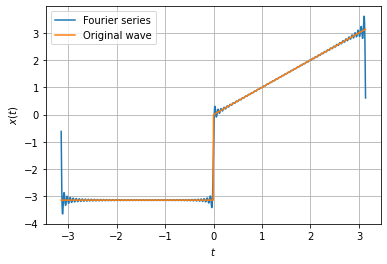
\includegraphics[width=0.8\columnwidth] {Gate_Assignment_4_Fig_3.png}
    \caption{$x(t)$ vs $t$}
    \label{Fourier series of x(t)}
\end{figure}
\end{frame}

\begin{frame}
\frametitle{}
We have a even periodic function having period $2\pi$ defined in $(0,2\pi)$ as follows :
\begin{align}
x(t)=  
\begin{cases}
t, & \text{if } 0 < t \leq \pi\\
2\pi-t, & \text{if } \pi \leq  t <  2\pi \nonumber
\end{cases}
\end{align}
The Fourier series of $x(t)$ is determined as follows:
\begin{align}
a_{0} &=\frac{1}{2\pi}\Bigg({\int_{-\pi}^{0}x(t)\, dt}+{\int_{0}^{\pi}x(t)\, dt}\Bigg)= \frac{\pi}{2} \nonumber \\
a_{k} &= \frac{1}{\pi}\Bigg({\int_{-\pi}^{0}x(t)\cos{kt}\, dt}+{\int_{0}^{\pi}x(t)\cos{kt}\, dt}\Bigg) \nonumber = \frac{2((-1)^{k}-1)}{\pi k^{2}}\nonumber \\
b_{k} &= \frac{1}{\pi}{\int_{-\pi}^{\pi}x(t)\sin{kt}\, dt} = 0\nonumber \\
\implies x(t) &= \frac{\pi}{2}-\frac{4}{\pi}\sum_{k=1}^{\infty}\frac{\cos{(2k-1)t}}{(2k-1)^{2}}
\end{align}
\end{frame}

\begin{frame}
\frametitle{}
\begin{figure}[!ht]
    \centering
    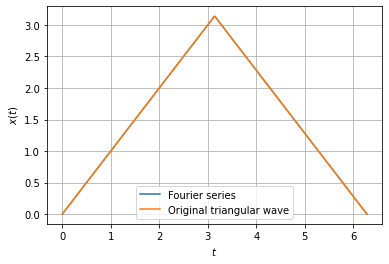
\includegraphics[width=0.8\columnwidth] {Gate_Assignment_4_Fig_4.png}
    \caption{$x(t)$ vs $t$}
    \label{Fourier series of x(t)}
\end{figure}
Hence the correct answer is option (3).
\end{frame}

\end{document}